\documentclass[10pt,a4paper,titlepage]{report}
\usepackage[utf8]{inputenc}
\usepackage{amsmath}
\usepackage{amsfonts}
\usepackage{amssymb}
\usepackage{graphicx}
\usepackage{xcolor}
\usepackage{minted}

\setlength{\arrayrulewidth}{0pt}
\setlength{\tabcolsep}{18pt}

\nonstopmode
\begin{document}

\newpage
\begin{center}
		\textbf{Project Report}\\\vspace{0.4cm}
on\\\vspace{1cm}
\begin{LARGE}
PHP Login Form
\end{LARGE}\\\vspace{0.4cm}
\textit{using LAMP Stack}\vspace{1cm}
\\
\textbf{Computer Science and Engineering}\\\vspace{1cm}
Submitted by\\\vspace{1cm}
\begin{tabular}{l|r}
	\textbf{Roll No.}&\textbf{Name}&
	38& Justine Biju&
	53& Rwithik Manoj&
\end{tabular}
\vfill
\textsc{College of Engineering, Trivandrum\\Semester 4}
\end{center}
\newpage
\tableofcontents

\chapter{Introduction}

LAMP is an archetypal model of web service stacks, named as an acronym of the names of its original four open-source components: the Linux operating system, the Apache HTTP Server, the MySQL relational database management system (RDBMS), and the PHP programming language. The LAMP components are largely interchangeable and not limited to the original selection. As a solution stack, LAMP is suitable for building dynamic web sites and web applications.
\newline
\par It is called a stack because each layer derives off its base layers. Linux, the OS forms the base layers. Apache, the web daemon, sits on top of the OS. The database, is hosted by the web daemon. PHP (or any scripting language) is used to drive and display all the data, and allow for user interaction.
\newline
\par The code of our project is hosted at https://github.com/justine05/foss-php
\section{Linux}
Linux is a family of open source Unix-like operating systems based on the Linux kernel, an operating system kernel first released on September 17, 1991 by Linus Torvalds. Linux is typically packaged in a Linux distribution (or distro for short). 

\par Popular Linux distributions include Debian, Fedora, and Ubuntu. Commercial distributions include Red Hat Enterprise Linux and SUSE Linux Enterprise Server. Desktop Linux distributions include a windowing system such as X11 or Wayland, and a desktop environment such as GNOME or KDE Plasma. Distributions intended for servers may omit graphics altogether, and include a solution stack such as LAMP. Because Linux is freely redistributable, anyone may create a distribution for any purpose. 

\section{Apache HTTP Server}
The role of LAMP's web server has been traditionally supplied by Apache, and has since included other web servers such as Nginx.
\par Apache is developed and maintained by an open community of developers under the auspices of the Apache Software Foundation. Released under the Apache License, Apache is open-source software. A wide variety of features are supported, and many of them are implemented as compiled modules which extend the core functionality of Apache. These can range from server-side programming language support to authentication schemes. 
\section{MySQL}
MySQL's original role as the LAMP's relational database management system (RDBMS) has since been alternately provisioned by other RDBMSs such as MariaDB or PostgreSQL, or even NoSQL databases such as MongoDB.
\par MySQL is a multithreaded, multi-user, SQL database management system (DBMS), acquired by Sun Microsystems in 2008, which was then acquired by Oracle Corporation in 2010. Since its early years, the MySQL team has made its source code available under the terms of the GNU General Public License, as well as under a variety of proprietary agreements. 
\par This application uses MariaDB, a community developed fork of MySQL, led by its original devs.
\section{PHP}
PHP's role as the LAMP's application programming language has also been performed by other languages such as Perl and Python. 
\par PHP is a server-side scripting language designed for web development but also used as a general-purpose programming language. PHP code is interpreted by a web server via a PHP processor module, which generates the resulting web page. PHP commands can optionally be embedded directly into an HTML source document rather than calling an external file to process data. It has also evolved to include a command-line interface capability and can be used in standalone graphical applications.

\chapter{The Database Schema}

\par The data base schema is as shown below\newline
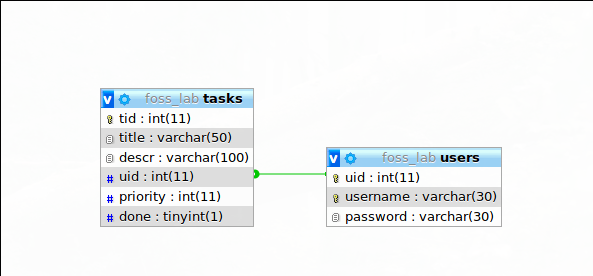
\includegraphics[width=\linewidth]{assets/schema.png}

A user table with the following attributes:
\begin{center}
	\begin{tabular}{|{2cm}|{2cm}|{2cm}|{2cm}|}
			uid& User ID& int& Primary Key, Auto Increment&
			username& Username& varchar(50)& Unique&
			password& Hash of the password& varchar(256)& 
	\end{tabular}
\end{center}

A tasks table with the following attributes:
\begin{center}
	\begin{tabular}{|{2cm}|{2cm}|{2cm}|{2cm}|}
			tid& Task ID& int& Primary Key, Auto Increment&
			title& Task Title& varchar(50)& &
			descr& Task Decription& varchar(100)& &
			uid& The User ID of the user& int& Foreign Key to users.uid&
			priority& Task Priority& int& &
			done& Whether the task is done& int& &
	\end{tabular}
\end{center}

\par The database is created using the phpmyadmin. The SQL query used is:

\begin{minted}[tabsize=4,breaklines]{php}
	CREATE TABLE users (
			id int(11) NOT NULL AUTO_INCREMENT,
			name varchar(30) NOT NULL,
			password varchar(512) NOT NULL,
			PRIMARY KEY (id),
			UNIQUE (username)
	) ENGINE=InnoDB DEFAULT CHARSET=utf8mb4;
\end{minted}

\begin{minted}[tabsize=4]{php}
	CREATE TABLE tasks (
			tid int(11) NOT NULL AUTO_INCREMENT,
			title varchar(50) NOT NULL,
			descr varchar(100) DEFAULT NULL,
			uid int(11) NOT NULL,
			priority int(11) NOT NULL DEFAULT 3,
			done tinyint(1) NOT NULL DEFAULT 0,
			PRIMARY KEY(tid),
			FOREIGN KEY (uid) REFERENCES users(uid)
	) ENGINE=InnoDB DEFAULT CHARSET=utf8mb4;
\end{minted}
\chapter{The To-Do Application}

\section{Introduction}
\par What we have made is a simple to-do application in which a user can login to see his/her personalized to-do list. 

\section{index.php}
\par This page is the front page of our application. It contains a login form and a link to the register page.

\begin{minted}[tabsize=4]{php}
	if (isset($_POST['submit']))
\end{minted}

\par This line checks if the user has come to the page after clicking the Login button. If it is the code checks if the inputs are not empty and are valid. 

\par If the inputs are valid, it gets the row from the database and verifies the password, redirecting to the {\color{red}tasks.php} page if the username and password match. If not, the corrosponding errors are printed onto the page.

\begin{minted}[tabsize=4,breaklines]{php}
$dbpass = mysqli_query($db,"SELECT password FROM users WHERE username = '$username' ");
$p = mysqli_fetch_array($dbpass)["password"];
if(empty($p)){
	$error = -1;
}
else if (password_verify($password, $p)){
	$error = 0;
	$_SESSION['username'] = $username;
	header('location: tasks.php');
}
\end{minted}

\section{register.php}
\par This page is used to register a new user. A register for is present in the page. This page contains similar code to check if the inputs are valid and if the user came to the page after clicking the Register button. Also checks if the password and the reentered password are the same. It also checks if the username already exists in the database. If everything is ok, the username and hashed password are inserted into the database. 
\par The user is then redirected to the login page.

\section{tasks.php}
\par It is the page that the user is redirected to after successful login. Here the user can veiw and add tasks to his personalized to-do list. Each task has a title, optional desription and a priority(default 3). The task can be marked as done. A task marked as done will have different CSS. 
\par There is also an option to cleared tasks from the list. It display the same page after a redirect via drop.php
\par Clicking the logout button, redirects the user to the login page, index.php, via a logout.php file. 

\section{logout.php}
\par This file clears the session and redirects to index.php file. 

\section{drop.php}
\par This file runs a query to drop all the tasks for the current user that are done.

\chapter{Conclusion}
\par We were able to successfully create a login page using php. First of all, we learnt the basics of PHP, SQL and HTML, we could complete the login page within 1 day. This project has helped us improve our knowledge of php and sql. We sincerely thank our teachers to give us an opportunity to form groups and complete the project as we could share our ideas and have a fruitful discussions!

\chapter{References}
\begin{enumerate}
		\item digitalocean.com
		\item stackoverflow.com
		\item w3schools.com
\end{enumerate}

\end{document}
